\documentclass[10pt]{beamer}
\usepackage{luatexja}
\usepackage{amsmath,amssymb}
\usepackage{bbm}
\usepackage{graphicx}
\usepackage{url}
% \usepackage{amsthm}
\usepackage{tikz}
\usetikzlibrary{arrows}
\usetikzlibrary{graphdrawing}
\usetikzlibrary{graphs}
\usegdlibrary{trees}
\newcommand{\bo}[1]{{\boldsymbol #1}}
\newcommand{\dx}{\,{\rm d}}
\newcommand{\difall}[2]{\frac{{\rm d}{#1}}{{\rm d}{#2}}}
\newcommand{\parpar}[2]{\frac{\partial{#1}}{\partial{#2}}}
\newcommand{\pmat}[1]{{\begin{pmatrix}#1\end{pmatrix}}}
\renewcommand{\div}{\mathop{\rm div}\nolimits}
\renewcommand{\thefootnote}{$\sharp$\arabic{footnote}}
\usetheme{Copenhagen}
\title{Piet処理系のスタック構造における\\B+木の高速性}
\author{sa8}
\begin{document}
\maketitle
% TODO: Pietのroll操作について言及
% TODO: 2分木で発生するキャッシュミスの恐れ
\section{平衡探索木とは?}
\begin{frame}
    \frametitle{2分探索木}
    \begin{block}{2分木}
        \begin{enumerate}
            \item \textbf{空}の木は2分木である.
            \item 次のいずれかを満足する節のみからなる木は, 2分木である:
                  \begin{itemize}
                      \item 子をもたない
                      \item 左の子のみをもつ
                      \item 右の子のみをもつ
                      \item 左右2つの子をもつ
                  \end{itemize}
        \end{enumerate}
    \end{block}
    各節の左の子を根とする部分木を{\bf 左部分木}と呼ぶ.{\bf 右部分木}も同様.
    \begin{block}{2分探索木}
        各節に持たせたデータが次の関係を満たす2分木

        \textsl{任意の節$\tt x$について, 左部分木の要素は節$\tt x$よりも小さく,
            右部分木に含まれる要素は節$\tt x$よりも大きい.}
    \end{block}
\end{frame}
\begin{frame}
    \frametitle{2分探索木}

    \begin{columns}[]
        \begin{column}{0.45\textwidth}
            \begin{alertblock}{弱点}
                木の高さが偏ったとき, \par
                探索性能が$O(\log N)$から$\Omega(N)$に悪化.
            \end{alertblock}
        \end{column}
        \begin{column}{0.55\textwidth}
            \begin{figure}
                \centering
                \begin{tikzpicture}[
                        >=stealth, every node/.style={circle, draw, minimum size=0.25cm},
                        etcetra/.style={circle,draw=black!30,minimum size=0.25cm},
                    ]
                    \graph[tree layout, grow=down, fresh nodes, level distance=0.2in, sibling distance=0.3in]
                    {
                    2->{
                    ,3->{
                    ,5->{
                    ,7->{
                    ,11->{
                    ,...[etcetra]}
                    }}}}};
                \end{tikzpicture}
                \caption{偏った2分木}
            \end{figure}
        \end{column}
    \end{columns}

\end{frame}
\begin{frame}
    \frametitle{平衡2分探索木}
    \begin{block}{平衡2分探索木}
        木の高さの偏りを抑える構造を持つ2分探索木.
    \end{block}
    \begin{exampleblock}{例}
        AVL木, Splay木, 赤黒木
    \end{exampleblock}

\end{frame}
\begin{frame}
    \frametitle{平衡2分木の例}
    \begin{figure}
        \includegraphics[width=\textwidth]{Images/RBTExample.pdf}
        \caption{赤黒木.データを葉にのみ格納.}
    \end{figure}

\end{frame}
\begin{frame}
    \frametitle{平衡多分木}

    \textbf{平衡2分木}の一般化.\vspace{1em}
    \underline{各親ノードが3以上の子を持ちうる}.

    \begin{figure}
        \includegraphics[width=\textwidth]{Images/QuadTreeExample.pdf}
        \caption{4分木の例.}
    \end{figure}

\end{frame}
\begin{frame}
    \frametitle{B木}

    \begin{block}{定義}
        多分岐の平衡木が, 条件
        \begin{itemize}
            \item 任意の葉の深さが等しい,
            \item 根を除く任意の節で, それの持つ枝の数が$\lceil m/2\rceil \ge k\ge m$個である,
            \item 根の持つ枝の数は$2\ge k \ge m$個である,
        \end{itemize}
        を満たすとき, この木をオーダー$m$の\textbf{B木}という.
    \end{block}

\end{frame}
\begin{frame}
    \frametitle{B+木\footnote{実装は\cite{kondo:2011}などを参照.}}

    レコードを葉にのみ持つ$\longrightarrow$葉と内部節との取扱いを区別できる.
    \begin{figure}
        \includegraphics[width=8cm,page=1]{Images/QuadTreeExample.pdf}
        \caption{B+木による配列実装の例.図は内部節のキーを省略している.}
    \end{figure}

    \begin{alertblock}{キーの内容}
        内部節のキーには, そこより若い部分木が持つ葉の数を用いる.
    \end{alertblock}

\end{frame}
\section{ベンチマーク}
\begin{frame}
    \frametitle{実験}

    \texttt{roll}コマンドのアルゴリズムを比較:
    \begin{itemize}
        \item 赤黒木
        \item 平衡2分探索木(オーダー$4$のB+木を使用)
        \item B+木(オーダー$4$超過, 今回はオーダー$64$)
        \item 配列のreverse
        \item 配列のswap
    \end{itemize}

    \cite{primenumber:2022}のベンチマークを実行:
    \texttt{push}, \texttt{pop}, \texttt{roll}のいずれかのクエリをランダムに$N$回呼び出し,
    平均処理時間\footnote{ここで``平均''とは,
        $\textrm{平均処理時間}:=\textrm{合計時間}/\textrm{クエリ数}$とする.}を比較.

\end{frame}
\begin{frame}
    \frametitle{結果}

    \begin{figure}
        \centering
        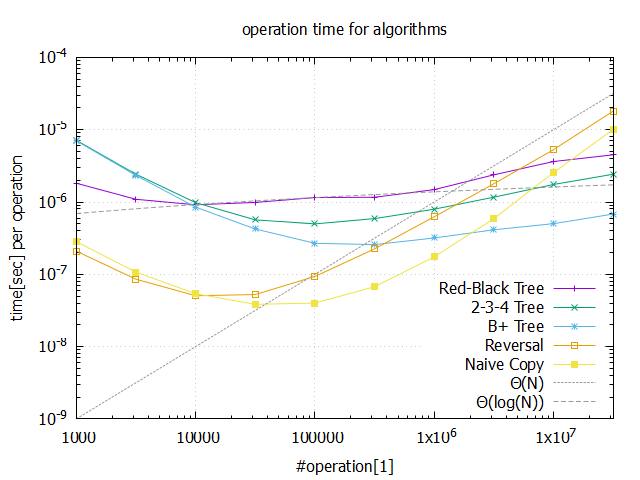
\includegraphics[width=0.7\textwidth]{algorithm.png}
        \caption{各アルゴリズムでの平均処理時間の比較.
        横軸がクエリ数$N$[1], 縦軸が平均処理時間[sec]を表す.}
    \end{figure}
\end{frame}
\begin{frame}
    \frametitle{\only<1>{結果}\only<2>{今後の課題}}

    \begin{columns}
        \begin{column}{0.4\textwidth}
            \begin{figure}
                \centering
                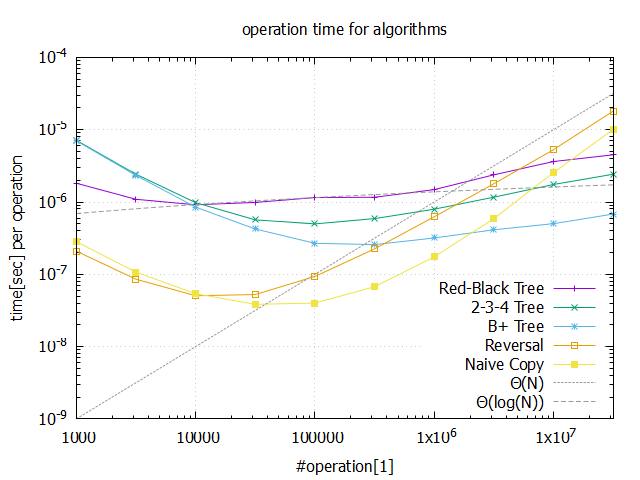
\includegraphics[width=1.0\textwidth, clip, trim=300 0 0 0]{algorithm.png}
                \caption{各アルゴリズムでの比較.}
            \end{figure}
        \end{column}
        \begin{column}{0.6\textwidth}
            \only<1>{
                \begin{itemize}
                    \item 配列法が予想通り平均$O(N)$.
                    \item $B+$木が他の平衡木より定数倍速い.
                    \item 平衡木法がいずれも$N>1\times {10}^6$で$\omega(\log N)$に悪化.
                          \begin{itemize}
                              \item キャッシュミスが原因?
                          \end{itemize}
                    \item 平衡木の性能が$N\lesssim 1\times{10}^6$で配列を超えられない.
                          \begin{itemize}
                              \item ノードのオブジェクト生成時間が定数倍のボトルネックになっている?
                              \item より最適化が可能?
                          \end{itemize}
                \end{itemize}
            }
            \only<2>{
                \begin{enumerate}
                    \item より効率的なデータ構造の検討
                          \begin{itemize}
                              \item 赤黒木, B+木は末尾参照に\\$\Omega(\log N)$かかる.
                              \item \textbf{2-3 Finger Tree}では\\償却$O(1)$で可能.
                          \end{itemize}
                \end{enumerate}
            }
        \end{column}
    \end{columns}
\end{frame}
\begin{frame}[allowframebreaks]{Reference}
    \scriptsize
    \beamertemplatetextbibitems
    \bibliographystyle{jplain}
    \bibliography{biblio}
\end{frame}
\end{document}